%!TEX root = ../main.tex

\chapter{Implementation} \label{chapt:implementation}

In this chapter we present the implementation details of the optimality test algorithm.
We give a brief explanation for each tool and we explain the safety and co-safety synthesizer.

\section{Optimality test algorithm}

The implemented optimality test algorithm is the one for the ASAP semantics.
That is because the best-effort semantics deals with variables of any domain. We could have used the set of natural numbers with $<$ as relation, but all arenas must be described in terms of boolean variables. 
Therefore, we would have had to consider only bounded integer variables and them to a boolean counter keeping up with the value of the corresponding variable.
It is not a problem at all, but it takes some time because we would also need to implement all operations between boolean counters.
On the contrary, in the ASAP semantics there are some tricks that we can use to implement it without introducing further boolean counters. 

The optimality test algorithm consists in various tools interacting each other.
These tools are: \lstinline{check_ltlspec}, \lstinline{_ebr2fsmv_time_limit}, \lstinline{_smv2fsmv}, \lstinline{fsmv2aig} and \lstinline{simplesynth}.
The first four software are implemented in the nuXmv software, while the last one is an external program.
All programs implemented as part of the plethora of nuXmv tools, they can be used from its CLI after reading the model.

The \lstinline{check_ltlspec} tool is an established tool in nuXmv which allows you to check $\ltl$ specifications on a model.
We use it to check whether the given formula is satisfied in the closed-loop between plant and controller.

The first tool made by us that we introduce is \lstinline{_ebr2fsmv_time_limit}, which must be executed after reading the model with the commands \lstinline{read_model} and \lstinline{go}.
This tool derives from \lstinline{_ebr2fsmv}, already introduced in \autoref{sec:ebr-ltl-synthesis}, which is useful to create the Deterministic Symbolic Safety Arena (DSA) from a $\ebrltl$ formula.
In contrast to the latter one, \lstinline{_ebr2fsmv_time_limit} creates the constrained DSA given a maximum number of steps $u$.
According to co-safety or safety synthesis, we build the arena in two different ways.
In the co-safety case we follow the construction given in \autoref{thm:asap-best-effort-co-safety}, exploiting a counter keeping up with the number of steps performed.
We do not need to introduce any further counter because the DSA of a $\ebrltl$ formula already has such type of counter, so we just need to check whether the counter is in the bound or not, as described in \autoref{lst:in-bound-co-safety}.
In the safety case, since we want to satisfy a formula in less than $u$ steps, we exploit this fact cutting off those sub-formulas which we are for sure not satisfiable in $u$ steps, so the monitor is built only for sub-formulas respecting the bound.
For example consider the construction of the monitor for $\phi = \ltlOr{\ltlX{p}}{(\ltlAnd{\ltlX{\ltlX{p}}}{\ltlX{q}})}$ with bound $u = 2$. 
We note that the sub-formula $\ltlX{\ltlX{p}}$ violates the bound and so it is for sure false, making also the conjunction false.
Therefore, the monitor for $\phi$ with bound $u=2$ is equivalent to the monitor for $\phi' = \ltlX{p}$.

Another important tool is \lstinline{_smv2fsmv}, which builds the monitor for a given plant.
It must be executed after reading the model with \lstinline{read_model} and \lstinline{go}.
The monitor plant construction is already explained in \autoref{lst:monitor-construction}.

After having built the two monitors and putting them together with the proper \lstinline{INVARSPEC} defining the set of safe states according to whether the formula is a co-safety or safety property, we are ready to convert the full arena in functional SMV format to AIGER format specifying the controllable variables, obtaining the game in AIGER format.
We can do it by the tool \lstinline{fsmv2aig}, previously implement it for the $\ebrltl$ specifications synthesis.
The only change we have brought to this tool are the initial changes to the AIGER version 2.0, introducing the possibility to assign a default value to latches.

The game in AIGER format is given in input to \lstinline{simplesynth}, which solves it.
This is an external program to nuXmv because, in principle, this piece of the tool-chain is interchangeable with any other synthesizer reading games in AIGER format.
There are many ways to solve safety and co-safety games and we do not want to limit the algorithm only to the one given by us.
Our safety and co-safety synthesizer is called \lstinline{simplesynth} and it allows to solve safety and co-safety games in AIGER format.
The symbolically algorithms exploited and how we represent the arena are described in \autoref{sec:reactive-synthesis}.
The only dependency of our synthesizer is the CUDD library, which is a library useful to manage BDDs.

The execution flow of the toolchain is the following: 
\begin{enumerate}[label=\enumpar]
    \item check whether the formula is satisfied in the closed-loop between plant and controller;
    \item regardless of the order, compute the monitor plant by \lstinline{_smv2fsmv} tool and the constrained formula monitor by \lstinline{_ebr2fsmv_time_limit} with \lstinline{u} as bound;
    \item do the synchronous product between the two monitors built before and add the proper \lstinline{INVARSPEC} according to the type of the formula we are synthesizing; 
    \item convert the arena from fsmv format to AIGER format indicating what are the controllable variables with the \lstinline{fsmv2aig} tool;
    \item solve the safety or co-safety game with any synthesizer accepting as input games described in AIGER format (e.g. \lstinline{simplesynth});
    \item if the previous step output is "realizable", then get the synthesized controller and output it. Otherwise, we output that there is no better controller. 
\end{enumerate}

If we consider the algorithm with the evaluation function, then we need to introduce more tools to solve the parameterized model checking problem: \lstinline{synth_param} and \lstinline{show_param_synth_problems}.
The first tool solve the parameterized model checking problem, while the second one show the solution of the problem just solved.
These two commands must be executed between steps $(1)$ and $(2)$, where we need to know the value of the bound $u$. The overall algorithm is depicted in \autoref{fig:asap-optimality}.

\begin{figure}[!htp]
    \centering
    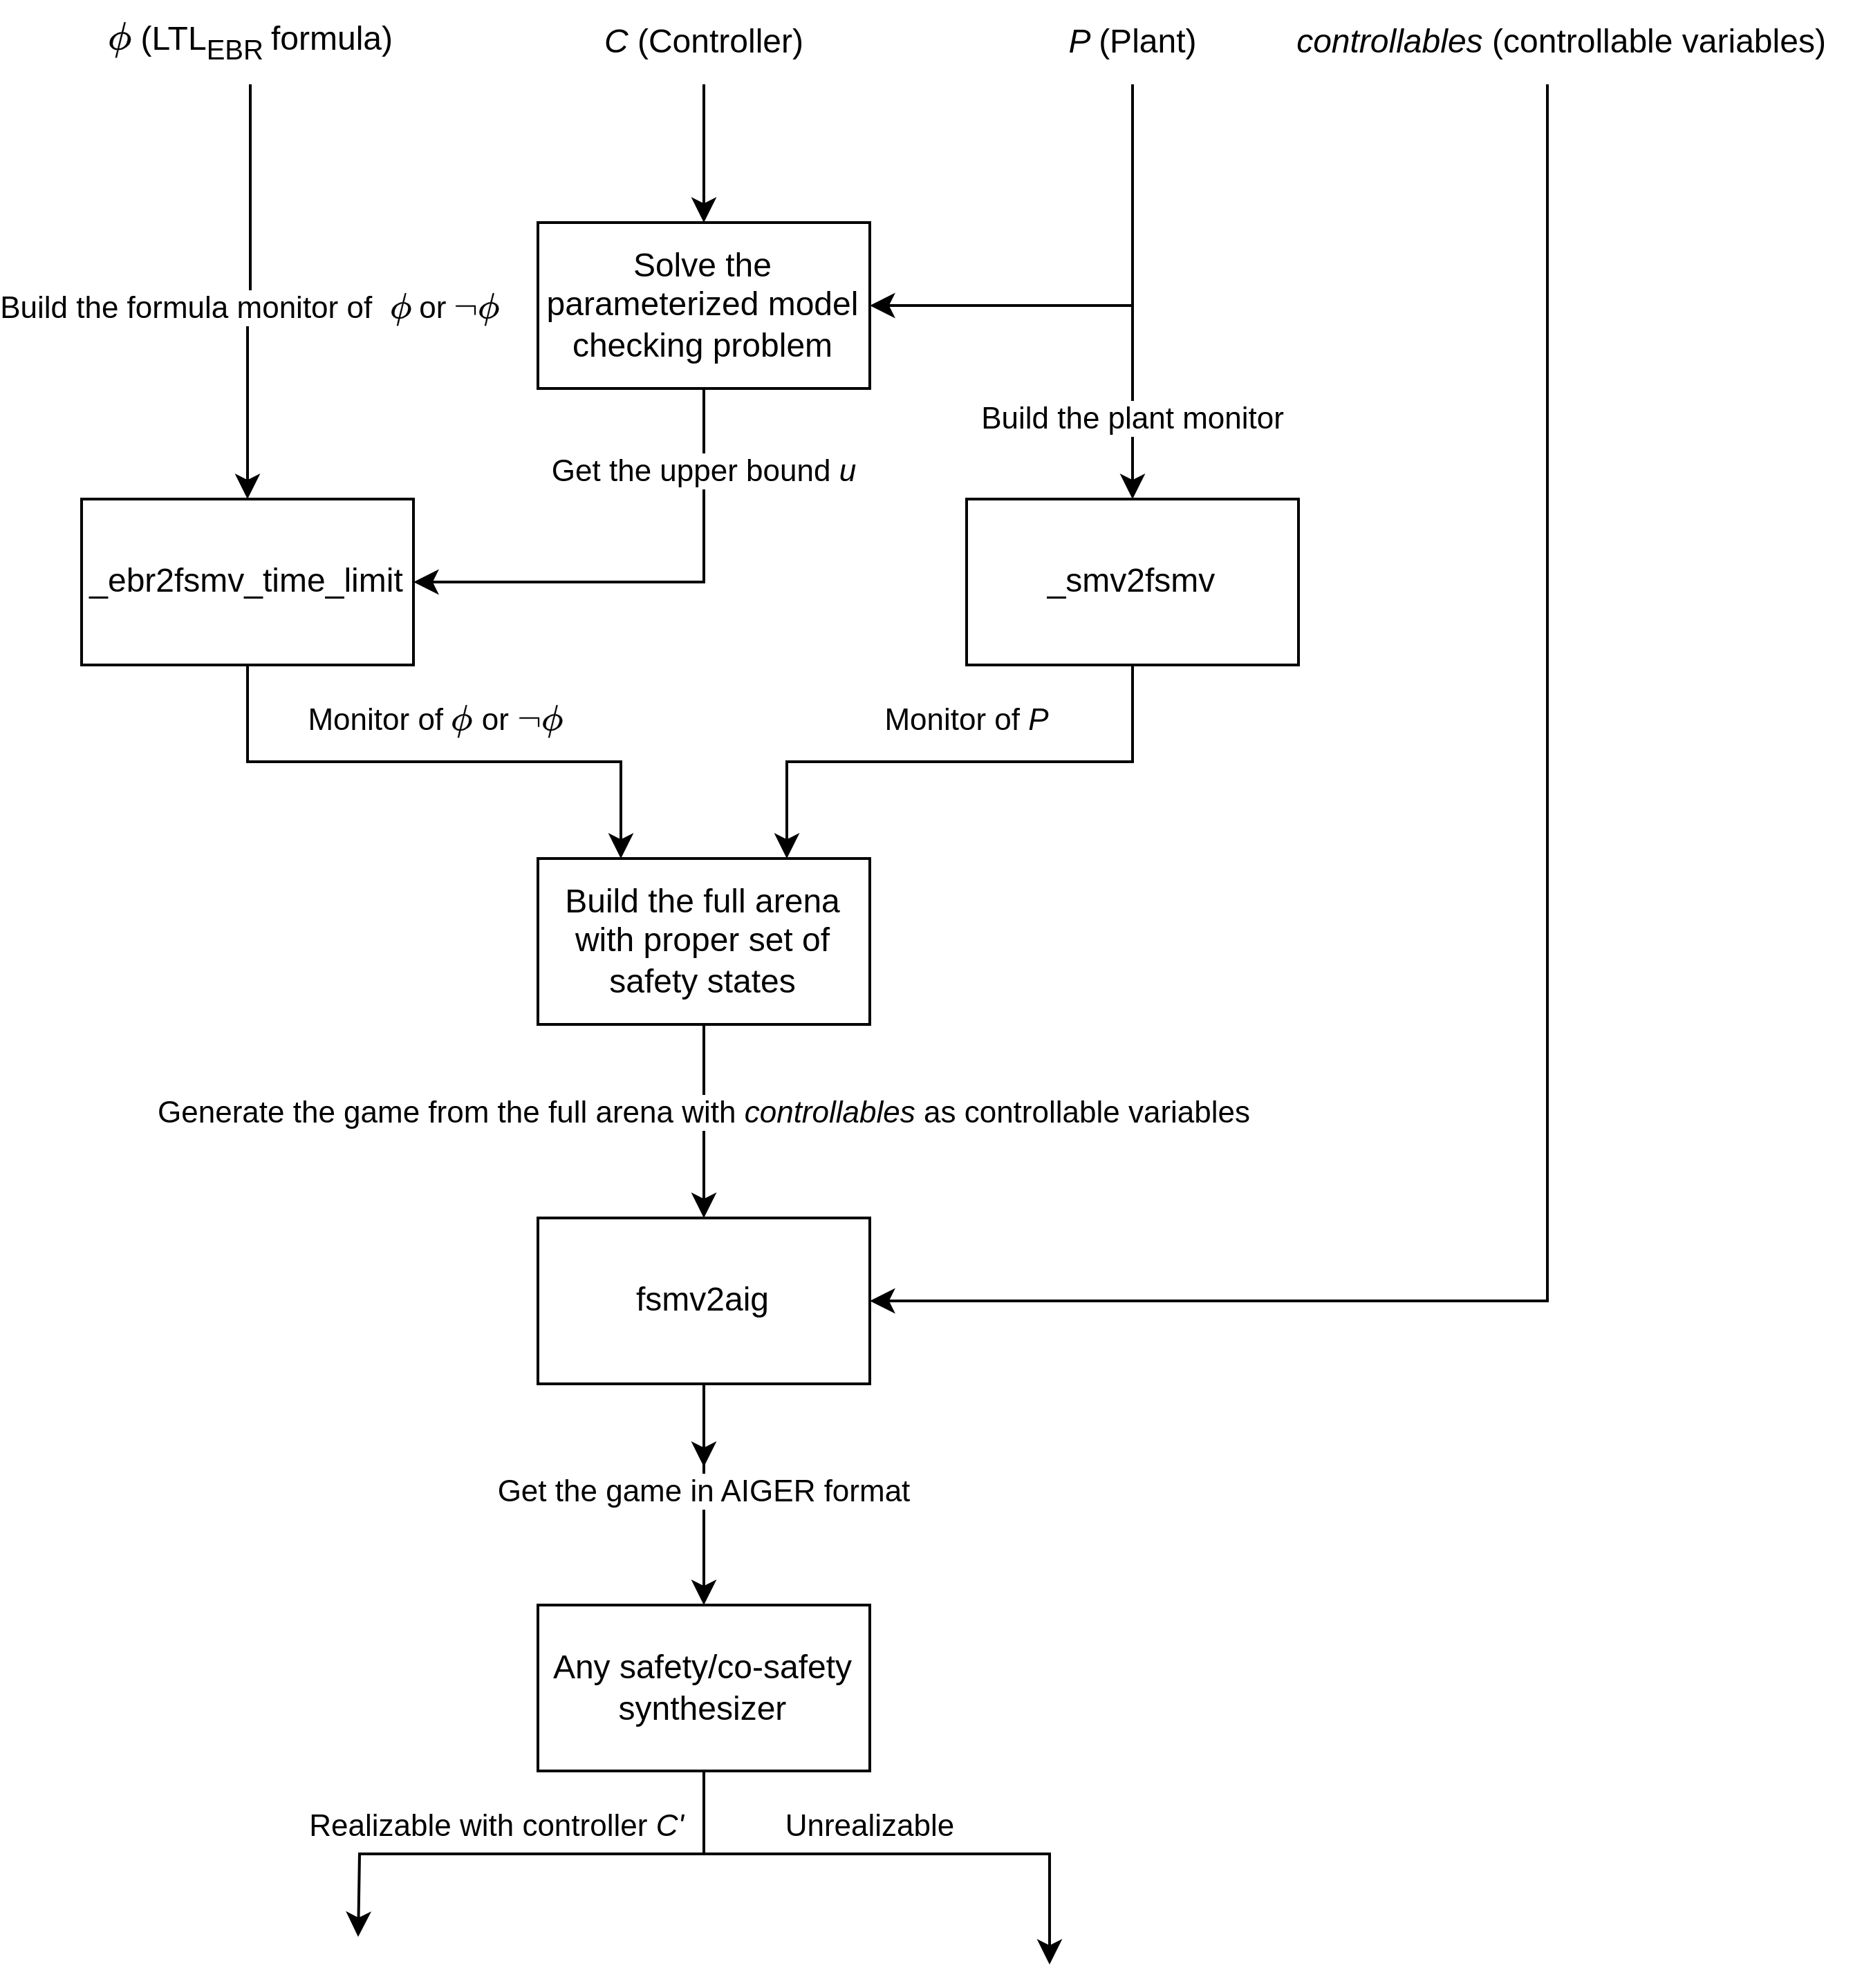
\includegraphics[width=0.6\linewidth]{figures/optimality-algorithm-asap.png}
    \caption{The optimality test algorithm for ASAP semantics graphically}
    \label{fig:asap-optimality}
\end{figure}

\section{Notable example}
In this section we show a notable example of the previous algorithm. It is useful to fix all concepts we have seen so far. As notable example we have chosen the ferryman puzzle which has already been introduced in \autoref{sec:smv} and for this reason we will not explain it again. 
Our aim is to satisfy the formula $\phi$ ASAP.
\begin{flalign*}
\ltlU{(\ltlImpl{(\ltlOr{\text{goat=wolf}}{\text{goat=cabbage}})}{\text{goat=man}})}{(\text{goat} \land \text{cabbage} \land \text{wolf} \land \text{man})}
\end{flalign*}

However, we need to make some changes to make it suitable for the optimality test algorithm.
First of all, we need to convert the plant to functional SMV format. 
The original plant is described through \lstinline{init} and \lstinline{next} statements, but it contains some atomic values and our tools cannot cope with them.
Therefore, we encode \lstinline{move} through two boolean variables, i.e. \lstinline{move0} and \lstinline{move1}, and each combination of them defines a move.

\begin{lstlisting}[language=smv, caption=Ferryman ASAP: plant in functional SMV format]
MODULE plant(move0,move1)
VAR
    man     : boolean;
    wolf    : boolean;
    goat    : boolean;
    cabbage : boolean;
DEFINE
    no_carry      := !move0 & !move1; -- move=e
    carry_goat    := move0  & !move1; -- move=g
    carry_wolf    := !move0 & move1;  -- move=w
    carry_cabbage := move0  & move1;  -- move=c
ASSIGN
    init(man)     := FALSE;
    init(goat)    := FALSE;
    init(wolf)    := FALSE;
    init(cabbage) := FALSE;
ASSIGN
next(cabbage) := case
  (carry_cabbage & (cabbage=man)) : !cabbage;
  TRUE : cabbage;
esac;
next(goat) := case
  (carry_goat & (goat=man)) : !goat;
  TRUE : goat;
esac;
next(wolf) := case
  (carry_wolf & (wolf=man)) : !wolf;
  TRUE : wolf;
esac;
next(man) := !man;
DEFINE
    safe_state := (goat=wolf | goat=cabbage) -> goat=man;
    goal := cabbage & goat & wolf & man;
\end{lstlisting}

After having defined the plant, let us define the controller.
For demonstration purposes we define a controller which is slower than the optimal one of two steps, introducing a delay at the beginning forcing an unnecessary carrying of the goat.

\begin{lstlisting}[language=smv, caption=Ferryman ASAP: slow controller]
MODULE SlowController(man, goat, wolf, cabbage)
VAR
-- possible moves
  move0 : boolean;
  move1 : boolean;
  delay : boolean;
INIT
  delay
TRANS
  next(delay) <-> (delay & !man)
ASSIGN
  move0 :=
    case
      !man:
        case
          man=cabbage & man=goat & man=wolf: TRUE;
          man=cabbage & man=goat: TRUE;
          man=cabbage & man=wolf: FALSE;
          man=cabbage: TRUE;
          man=goat & man=wolf: FALSE;
          man=goat : TRUE;
          man=wolf : FALSE;
          TRUE : FALSE;
        esac;
      TRUE:
        case
          delay : TRUE;
          man=cabbage & man=goat: TRUE;
          man=goat & man=wolf: TRUE;
          TRUE: FALSE;
        esac;
    esac;
ASSIGN
  move1 :=
    case
      !man:
        case
          man=cabbage & man=goat & man=wolf: FALSE;
          man=cabbage & man=goat: TRUE;
          man=cabbage & man=wolf: TRUE;
          man=cabbage: TRUE;
          man=goat & man=wolf: TRUE;
          man=goat : FALSE;
          man=wolf : TRUE;
          TRUE : FALSE;
        esac;
      TRUE:
        case
          delay : FALSE;
          man=cabbage & man=goat: TRUE;
          man=goat & man=wolf: FALSE;
          TRUE: FALSE;
        esac;
    esac;
\end{lstlisting}

We can now compute the upper-bound $u$ required by the algorithm to find out whether there exists a controller which enforces the formula in a smaller number of steps.
To discover this bound we need to solve a parameterized model checking problem on the maximum number of steps that can be performed enforcing the formula and look for the minimum value among those values.
In SMV a parameterized model checking problem is formulated in the following way:
\begin{lstlisting}[language=smv, caption=Ferryman ASAP: parameterized model checking problem with until operator]
MODULE main
VAR
  p: Plant(c.move);
  c: SlowController(p.cabbage, p.goat, p.wolf, p.man);
-- Parameterized model checking problem
VAR time: 0..10;
FROZENVAR maxtime: 0..10;
ASSIGN
  init(time) := 0;
  next(time) := case time < 10 : time + 1; TRUE: time; esac;
  PARSYNTH r := { maxtime | VALID (p.safe_state U (p.goal & time<=maxtime)) };
\end{lstlisting}

Basically, we introduce two variables: \lstinline{time} and \lstinline{maxtime}.
The first one counts the number of steps already performed, while the second one is the parameter to synthesize. So we look for the fixed values of \lstinline{maxtime} for which the formula is satisfied.
It is easy to see that when \lstinline{maxtime} is too low we cannot satisfy the right side of until temporal operator and so the whole formula is false.
For efficiency reasons we convert this formula to an equivalent safety formula. That is because, as we have already seen, is possible to reduce the model checking of safety formulas to an invariant verification problem, which is more efficient.
We rewrite the formula in terms of release (in NuSMV the release symbol is \lstinline{V}), where whenever we exceed the time we need to satisfy the goal as well, otherwise the whole formula will be false.

\begin{lstlisting}[language=smv, caption=Ferryman ASAP: parameterized model checking problem with release operator]
PARSYNTH r := { maxtime | VALID (p.goal V (p.safe_state & time<=maxtime)) };
\end{lstlisting}

By executing the following commands to solve the parameterized model checking problem in the nuXmv CLI, we can see that the least upper-bound to \lstinline{maxtime} is $9$.
Therefore we can state that \lstinline{Plant} is satisfied ASAP by \lstinline{ControllerSlow} in $9$ steps.
\begin{lstlisting}[language=bash, caption=Ferryman ASAP: commands to execute to solve the parameterized model checking problem]
nuXmv > go_bmc
nuXmv > synth_param -a ic3 -s -l -c
nuXmv > show_param_synth_problems  
There is 1 param synth problem:
001: SYNTH r := { maxtime | VALID !(!p.goal U !(p.safe_state & time <= maxtime)) }, region: (maxtime = 10 | maxtime = 9)
\end{lstlisting}

Now we look for a controller which can satisfy the formula in less steps.
First of all we generate the plant monitor by \lstinline{_smv2fsmv} tool. 

\begin{lstlisting}[language=smv, caption=Ferryman ASAP: plant monitor]
MODULE monitor_0(move0,move1,man,wolf,goat,cabbage)
VAR
   MON_0_ERROR_cabbage : boolean;
   MON_0_SIM_cabbage : boolean;
   MON_0_ERROR_goat : boolean;
   MON_0_SIM_goat : boolean;
   MON_0_ERROR_wolf : boolean;
   MON_0_SIM_wolf : boolean;
   MON_0_ERROR_man : boolean;
   MON_0_SIM_man : boolean;
DEFINE
   MON_0_ERROR := (MON_0_ERROR_wolf | (MON_0_ERROR_man | (MON_0_ERROR_cabbage | MON_0_ERROR_goat)));
   no_carry := (!move0 & !move1);
   carry_goat := (move0 & !move1);
   carry_wolf := (!move0 & move1);
   carry_cabbage := (move0 & move1);
ASSIGN
   init(MON_0_ERROR_wolf) := FALSE;
   init(MON_0_SIM_wolf) := FALSE;
   init(MON_0_ERROR_man) := FALSE;
   init(MON_0_SIM_man) := FALSE;
   init(MON_0_ERROR_cabbage) := FALSE;
   init(MON_0_SIM_cabbage) := FALSE;
   init(MON_0_ERROR_goat) := FALSE;
   init(MON_0_SIM_goat) := FALSE;
ASSIGN
   next(MON_0_SIM_wolf) := case
    (carry_wolf & (MON_0_SIM_wolf<->MON_0_SIM_man)) : !MON_0_SIM_wolf;
    TRUE : MON_0_SIM_wolf;
   esac;
   next(MON_0_SIM_cabbage) := case
    (carry_cabbage & (MON_0_SIM_cabbage <-> MON_0_SIM_man)) : !MON_0_SIM_cabbage;
    TRUE : MON_0_SIM_cabbage;
   esac;
   next(MON_0_SIM_goat) := case
    (carry_goat & (MON_0_SIM_goat <-> MON_0_SIM_man)) : !MON_0_SIM_goat;
    TRUE : MON_0_SIM_goat;
   esac;
   next(MON_0_SIM_man) := !MON_0_SIM_man;
ASSIGN
   next(MON_0_ERROR_man) := (MON_0_ERROR_man | (MON_0_SIM_man != man));
   next(MON_0_ERROR_wolf) := (MON_0_ERROR_wolf | (MON_0_SIM_wolf != wolf));
   next(MON_0_ERROR_cabbage) := (MON_0_ERROR_cabbage | (MON_0_SIM_cabbage != cabbage));
   next(MON_0_ERROR_goat) := (MON_0_ERROR_goat | (MON_0_SIM_goat != goat));
\end{lstlisting}

Then, since $\phi$ is a co-safety formula, we negate it and generate the monitor of the negated formula by \lstinline{_ebr2fsmv_time_limit} tool with bound $8$.

\begin{lstlisting}[language=smv, caption=Ferryman ASAP: formula monitor with bound $8$]
MODULE ltl_spec_0(move0,move1,man,wolf,goat,cabbage)
VAR
   EBR_0_PAST_1 : boolean;
   EBR_0_ERROR_0 : boolean;
   EBR_0_COUNTER_4 : boolean;
   EBR_0_COUNTER_3 : boolean;
   EBR_0_COUNTER_2 : boolean;
   EBR_0_COUNTER_1 : boolean;
   EBR_0_COUNTER_0 : boolean;
DEFINE
   EBR_0_ERROR := (!EBR_0_EXPIRED & EBR_0_ERROR_0);
   EBR_0_EXPIRED := !(!EBR_0_COUNTER_4 & (!EBR_0_COUNTER_3 | (!EBR_0_COUNTER_2 & !EBR_0_COUNTER_1)));
ASSIGN
   init(EBR_0_PAST_1) := FALSE;
   init(EBR_0_ERROR_0) := FALSE;
   init(EBR_0_COUNTER_4) := FALSE;
   init(EBR_0_COUNTER_3) := FALSE;
   init(EBR_0_COUNTER_2) := FALSE;
   init(EBR_0_COUNTER_1) := FALSE;
   init(EBR_0_COUNTER_0) := FALSE;
ASSIGN
   next(EBR_0_PAST_1) := case
    ((((!goat | wolf) & (!wolf | goat)) | ((!goat | cabbage) & (!cabbage | goat))) & ((goat & !man) | (man & !goat))) : TRUE;
    EBR_0_PAST_1 : TRUE;
   TRUE : FALSE;
esac;
ASSIGN
   next(EBR_0_ERROR_0) := case
    (!EBR_0_ERROR_0 & EBR_0_PAST_1) : FALSE;
    (!EBR_0_ERROR_0 & (((((!goat | wolf) & (!wolf | goat)) | ((!goat | cabbage) & (!cabbage | goat))) & ((goat & !man) | (man & !goat))) & (((!cabbage | !goat) | !wolf) | !man))) : FALSE;
    (!EBR_0_ERROR_0 & (((!cabbage | !goat) | !wolf) | !man)) : FALSE;
    TRUE : TRUE;
   esac;
ASSIGN
   next(EBR_0_COUNTER_4) := (((((EBR_0_COUNTER_0 & EBR_0_COUNTER_1) & EBR_0_COUNTER_2) & EBR_0_COUNTER_3) & EBR_0_COUNTER_4) | ((EBR_0_COUNTER_3 & (EBR_0_COUNTER_2 & (EBR_0_COUNTER_1 & EBR_0_COUNTER_0))) <-> !EBR_0_COUNTER_4));
ASSIGN
   next(EBR_0_COUNTER_3) := (((((EBR_0_COUNTER_0 & EBR_0_COUNTER_1) & EBR_0_COUNTER_2) & EBR_0_COUNTER_3) & EBR_0_COUNTER_4) | ((EBR_0_COUNTER_2 & (EBR_0_COUNTER_1 & EBR_0_COUNTER_0)) <-> !EBR_0_COUNTER_3));
ASSIGN
   next(EBR_0_COUNTER_2) := (((((EBR_0_COUNTER_0 & EBR_0_COUNTER_1) & EBR_0_COUNTER_2) & EBR_0_COUNTER_3) & EBR_0_COUNTER_4) | ((EBR_0_COUNTER_1 & EBR_0_COUNTER_0) <-> !EBR_0_COUNTER_2));
ASSIGN
   next(EBR_0_COUNTER_1) := (((((EBR_0_COUNTER_0 & EBR_0_COUNTER_1) & EBR_0_COUNTER_2) & EBR_0_COUNTER_3) & EBR_0_COUNTER_4) | (EBR_0_COUNTER_0 <-> !EBR_0_COUNTER_1));
ASSIGN
   next(EBR_0_COUNTER_0) := (((((EBR_0_COUNTER_0 & EBR_0_COUNTER_1) & EBR_0_COUNTER_2) & EBR_0_COUNTER_3) & EBR_0_COUNTER_4) | !EBR_0_COUNTER_0);
\end{lstlisting}

At this point we have all required monitors with the corresponding errors variables, i.e. \lstinline{EBR_0_ERROR} for the monitor of the negated formula and \lstinline{MON_0_ERROR} for the monitor of the plant.
We make synchronous product between the two monitors and set the correct \lstinline{INVARSPEC}.
Note that, contrary to how we defined this part in \autoref{sec:reduction-to-synthesis}, we do not need the additional variable \lstinline{in_bound} because we force the bound directly in the formula monitor with \lstinline{EBR_0_EXPIRED}.

\begin{lstlisting}[language=smv, caption=Ferryman ASAP: main module]
MODULE main
IVAR
    man : boolean;
    goat : boolean;
    wolf : boolean;
    cabbage : boolean;
    move0 : boolean;
    move1 : boolean;
VAR
   m : monitor_0(move0,move1,man,wolf,goat,cabbage);
   p : ltl_spec_0(move0,move1,man,wolf,goat,cabbage);
INVARSPEC !m.MON_0_ERROR & !p.EBR_0_ERROR
\end{lstlisting}

Finally we have the whole arena which can be converted to AIGER format by \lstinline{fsmv2aig} tool where we specify the controllable variables, i.e. \lstinline{move0} and \lstinline{move1}.
We end up with the game in AIGER format which can be solved by any synthesizer.
The output of the execution of \lstinline{simplesynth} synthesizer on the game is that the game is realizable and it provides us a new controller which is better than the given one.
Indeed, if we solve the parameterized model checking on the closed-loop of the plant with the new controller, we see that the formula is satisfied in $7$ steps instead of the previous $9$ steps.
Moreover, if we repeat the whole algorithm with the new controller, we note that there is no other controller better than the current one and therefore we state that the synthesized controller is also optimal.
